\documentclass[11pt]{article}

\usepackage[margin=2cm, a4paper]{geometry}	%2cm page margin
\usepackage{fancyhdr}						%use fancy headers
\usepackage{graphicx}						%use images
\usepackage{textcomp}						%used for textdegree command
\usepackage[hidelinks]{hyperref}            %used for clickable references
\usepackage{draftwatermark}
\SetWatermarkLightness{ 0.9 }
\SetWatermarkText{Preliminary}
\SetWatermarkScale{ 4 }

%DPTECHNICS datasheet variables
\newcommand{\dptproduct}{Walter - WiFi/BLE/NB-IoT/LTE-M module}

\newcommand{\textoverline}[1]{$\overline{\mbox{#1}}$}

%page footers and headers settings
\pagestyle{fancy}
\fancyhead{}
\fancyfoot{}
\fancyhead[LO,LE]{ {\bf \dptproduct}}
\fancyfoot[R]{\thepage}
\fancyfoot[L]{QuickSpot - 2023}
\renewcommand{\footrulewidth}{0.4pt}
\renewcommand\familydefault{\sfdefault}
\setlength{\parindent}{0pt}

\begin{document}
\begin{titlepage}
\hfill
\includegraphics[width=8cm]{logo.pdf}\\

\hfill {\bf \Large  \dptproduct}\\[-3mm]

\hfill {\Large Preliminary Datasheet}

\vfill
\rule{487pt}{1pt}

\hfill Revision 0.4 - \today
\end{titlepage}
\section{General information}
Walter is an ESP32-S3 based IoT board that offers WiFi, Bluetooth 5 (LE), cellular CAT M1/NB1/NB2 and GNSS connectivity. 

\section{Features}
Walter is based on an ESP32-S3-WROOM-1-N16R2 module with an on-board Sequans GM02SP modem.
This combination makes Walter a unique development board that offers a rich feature-set which include but is not limited to:
\begin{itemize}
	\item CPU: Xtensa Dual-core 32-bit LX7 CPU (ESP32-S3 SoC)
	\item RAM: 2MB (Quad SPI) PSRAM
	\item Flash: 16MB (Quad SPI) Flash memory
	\item WiFi: 150Mbps(n) 802.11 WiFi b/g/n with on-board antenna
	\item LTE: CAT M1/NB1/NB2 (GM02SP module)
	\item GPS: GPS, GNSS Constellation support (GM02SP module)
	\item Bluetooth: 2Mbps Bluetooth 5 (LE), Bluetooth Mesh
	\item 24 physical GPIO pins 
\end{itemize}

\section{Electrical characteristics}
For the most reliable use and stability of the module we advice to use the typical ratings. We do not guarantee the correct functioning of the device outsite the minimum and maxium range of the module. 
\begin{center}
\renewcommand{\arraystretch}{1.5}
\begin{tabular}{|p{5cm}|c|c|c|c|}
\hline
{\bf Parameter} & {\bf Units} & {\bf Minimum rating} & {\bf Typical rating} & {\bf Maximum rating} \\
\hline
\hline
DC Supply Voltage & V & 3.0 & 5.0 & 5.5 \\
\hline
Digital I/O Voltage & V & 2.64 & 3.3 & 3.6 \\
\hline
Power consumption @3.3V & A & -- & -- & 1.5 \\
\hline
3.3V output & A & -- & -- & 0.25 \\
\hline
\end{tabular}
\end{center}

\newpage
\section{Interfaces}
Walter provides a total of 28 physical pins (3 power, 1 strapping pin and 24 I/O pins) to interface with external parts. This chapter provides information about these pins as well as internally connected pins and the testpoints located at the bottom of the board.\\

Power supply pins and their details are available in section \ref{power} about the power characteristics.\\

For more information about specific pins regarding the ESP32-S3 Wroom module or the Sequans GM02SP module, please refer to the datasheet of the corresponding module.

\subsection{Pin Assignment} \label{pin_assigment}

\begin{figure}[h]
    \centering
    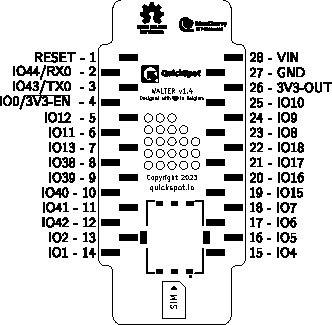
\includegraphics[height=14cm]{walter-pinout-topview.pdf}
    \caption{Walter pinout (top view)}
    \label{fig:walter_pin_assignment}
\end{figure}
\newpage
\subsubsection{External Pins} \label{external_pins}
Table \ref{table_exteral_pin} contains the description of the physical pins on Walter available on the underside of the board. \\
The order of this table, in reference to the board, is top to bottom and left to right.\\
\renewcommand{\arraystretch}{1.5}
\begin{table}[!h]
\begin{center}
\begin{tabular}{|c|c|c|c|c|p{9.5cm}|}
\hline
{\bf Pin} & {\bf Function} & \multicolumn{1}{c|}{\bf ESP pin} & \multicolumn{1}{c|}{\bf Input/Output} & \multicolumn{1}{c|}{\bf Description} \\
\hline
\hline
1 & RESET & EN & input & ESP32 reset with 10k pullup \\
\hline
2 & IO44/RX0 & RXD0 & bidirectional & ESP32 UART0 Receive \\
\hline
3 & IO43/TX0 & TXD0 & bidirectional & ESP32 UART0 Transmit \\
\hline
4 & \textoverline{DFU}/\textoverline{3V3\_EN} & IO0 & bidirectional & DFU when low on boot and 3V3 output enable \\
\hline
5 & IO12 & IO12 & bidirectional & General purpose I/O \\
\hline
6 & IO11 & IO11 & bidirectional & General purpose I/O \\
\hline
7 & IO13 & IO13 & bidirectional & General purpose I/O \\
\hline
8 & IO38 & IO38 & bidirectional & General purpose I/O \\
\hline
9 & IO39 & IO39 & bidirectional & General purpose I/O \\
\hline
10 & IO40 & IO40 & bidirectional & General purpose I/O \\
\hline
11 & IO41 & IO41 & bidirectional & General purpose I/O \\
\hline
12 & IO42 & IO42 & bidirectional & General purpose I/O \\
\hline
13 & IO2 & IO2 & bidirectional & General purpose I/O \\
\hline
14 & IO1 & IO1 & bidirectional & General purpose I/O \\
\hline
15 & IO4 & IO4 & bidirectional & General purpose I/O \\
\hline
16 & IO5 & IO5 & bidirectional & General purpose I/O \\
\hline
17 & IO6 & IO6 & bidirectional & General purpose I/O \\
\hline
18 & IO7 & IO7 & bidirectional & General purpose I/O \\
\hline
19 & IO15 & IO15 & bidirectional & General purpose I/O \\
\hline
20 & IO16 & IO16 & bidirectional & General purpose I/O \\
\hline
21 & IO17 & IO17 & bidirectional & General purpose I/O \\
\hline
22 & IO18 & IO18 & bidirectional & General purpose I/O \\
\hline
23 & IO8 & IO8 & bidirectional & General purpose I/O \\
\hline
24 & IO9 & IO9 & bidirectional & General purpose I/O \\
\hline
25 & IO10 & IO10 & bidirectional & General purpose I/O \\
\hline
26 & 3V3 OUT & N/A & power output & Switchable 3.3VDC output \\
\hline
27 & GND & GND & power ground & GND connection \\
\hline
28 & VIN & N/A & power input & DC Power input port\\
\hline
\end{tabular}
\caption{\label{table_exteral_pin}Walter pin definitions}
\end{center}
\end{table}
\newpage

\subsubsection{Internal Pins} \label{internal_pins}
Table \ref{table_interal_pin} contains the pin descriptions of the internally connected GPIO pins on Walter. These are necessary for either communication between components on the board or reserved for other purposes and thus not available for external use.

\begin{table}[!h]
    \centering
    \begin{tabular}{|c|p{9.5cm}|}
    \hline
    {\bf ESP pin} & \multicolumn{1}{c|}{\bf Description} \\
    \hline
    \hline
    IO19 & USB D-\\
    \hline
    IO20 & USB D+\\
    \hline
    IO46 & LTE\_WAKE0 \\
    \hline
    IO48 & LTE\_UART0\_TX (See \ref{lte_uart})\\
    \hline
    IO14 & LTE\_UART0\_RX (See \ref{lte_uart})\\
    \hline
    IO21 & LTE\_UART0\_RTS (See \ref{lte_uart})\\
    \hline
    IO47 & LTE\_UART0\_CTS (See \ref{lte_uart})\\
    \hline
    IO45 & LTE\_RESET\\
    \hline
    \end{tabular}
    \caption{\label{table_interal_pin}Walter Internal Pin Definitions}
\end{table}

\newpage
\subsubsection{Testpoints} \label{testpoints}
Walter contains 22 testpoints on the bottom of the board that serve multiple purposes. You can use these pins for debugging, interfacing and/or flashing of the Sequans GM02SP and the ESP32-S3-WROOM module.
\begin{figure}[h]
    \centering
    
\includegraphics[height=5cm]{walter-testpoints.pdf}
    \caption{Walter testpoints}
    \label{fig:testpoints}
\end{figure}

\begin{center}
\begin{tabular}{|c|p{9.5cm}|}
    \hline
    {\bf Number} & \multicolumn{1}{c|}{\bf Description} \\
    \hline
    \hline
    1 & Sequans GM02SP JTAG TDO\\
    \hline
    2 & Sequans GM02SP JTAG TCK\\
    \hline
    3 & Sequans GM02SP JTAG TRSTN\\
    \hline
    4 & Sequans GM02SP JTAG TMS\\
    \hline
    5 & Sequans GM02SP JTAG TDI\\
    \hline
    6 & Sequans GM02SP PS status\\
    \hline
    7 & Sequans GM02SP RES/FFF\_FFH \\
    \hline
    8 & Sequans GM02SP RX0 \\
    \hline
    9 & Sequans GM02SP TX0 \\
    \hline
    10 & Sequans GM02SP TX1 \\
    \hline
    11 & Sequans GM02SP RX1 \\
    \hline
    12 & Sequans GM02SP RX2 \\
    \hline
    13 & Sequans GM02SP CTS0 \\
    \hline
    14 & Sequans GM02SP RTS0 \\ 
    \hline
    15 & Sequans GM02SP CTS1 \\
    \hline
    16 & Sequans GM02SP RTS1 \\
    \hline
    17 & Sequans GM02SP TX2 \\
    \hline
    18 & Walter input power \\
    \hline
    19 & 3V3 output (not switched) \\
    \hline
    20 & Sequans GM02SP 1V8 output \\
    \hline
    21 & Ground \\
    \hline
    22 & ESP32-S3 GPIO3 (strapping pin)\\
    \hline
\end{tabular}
\end{center}

\begin{figure}[h]
    \centering
    
\includegraphics[height=8cm]{walter-testpoints-named.pdf}
    \caption{Bottom view of the Walter testpoints with their connection names.}
    \label{fig:testpoints}
\end{figure}

\subsubsection{Others}
Not all pins of the ESP32-S3 and Sequans GM02SP on Walter are internally connected, available through physical pins or testpoints. These pins are either reserved for use by the component itself or deemed not necessary to be available externally.

\subsection{Sequans GM02SP UARTs} \label{lte_uart}
The Sequans GM02SP module has 3 hardware UART interfaces. Only UART0 is connected to the ESP32-S3 Wroom Module on Walter as shown in Table \ref{table_interal_pin}. Communication between modules is possible with AT-commands. Please refer to the corresponding AT command reference manual of the Sequans GM02SP for all possible AT-commands. The UARTs have the following functionality by default:
\begin{itemize}
	\item UART0 (115200@8N1 with HW handshaking): used for AT commands.
	\item UART1 (921600@8N1 with HW handshaking): used for manual firmware updates and/or custom software installation.
	\item UART2 (115200@8N1 no HW handshaking): console log output.
\end{itemize}

Please not that any UART host should be connected as follows:
\begin{itemize}
	\item \verb+RX <-> RX+
	\item \verb+TX <-> TX+
	\item \verb+RTS <-> RTS+
	\item \verb+CTS <-> CTS+
\end{itemize}
\section{Electrical and RF Characteristics} \label{power_rf_characteristics}
\subsection{Power} \label{power}
\subsubsection{Power Input}
Walter can be powered either by connecting a USB-C cable or via the VIN pin (see pinout \ref{external_pins}).\\

\textbf{DO NOT} power Walter with both the USB-C connection and the VIN-pin! This can lead to seriously damaging the board and external peripherals connected to it!
\subsubsection{Power Output}
Walter contains a Texas Instruments LM3281YFQR DC-DC Converter which takes power from either the USB-C port or the VIN-pin and converts it to a regulated +3.3VDC supply.
\subsubsection{Power Consumption}
\subsection{GPIO} \label{gpio}
All GPIO pins exposed via the physical pin headers on Walter are 3.3V resistant. If you want to connect 5V or other forms of logic, please use a suitable logic level converter or voltage divider.\\

Please reference the corresponding datasheets for all minimum, maximum and typical ratings of I/O pins of the ESP32-S3-WROOM or Sequans GM02SP Modules that may or may not be exposed on the Walter Development Board.

\newpage
\section{Mechanical information}
\begin{figure}[h]
    \centering
    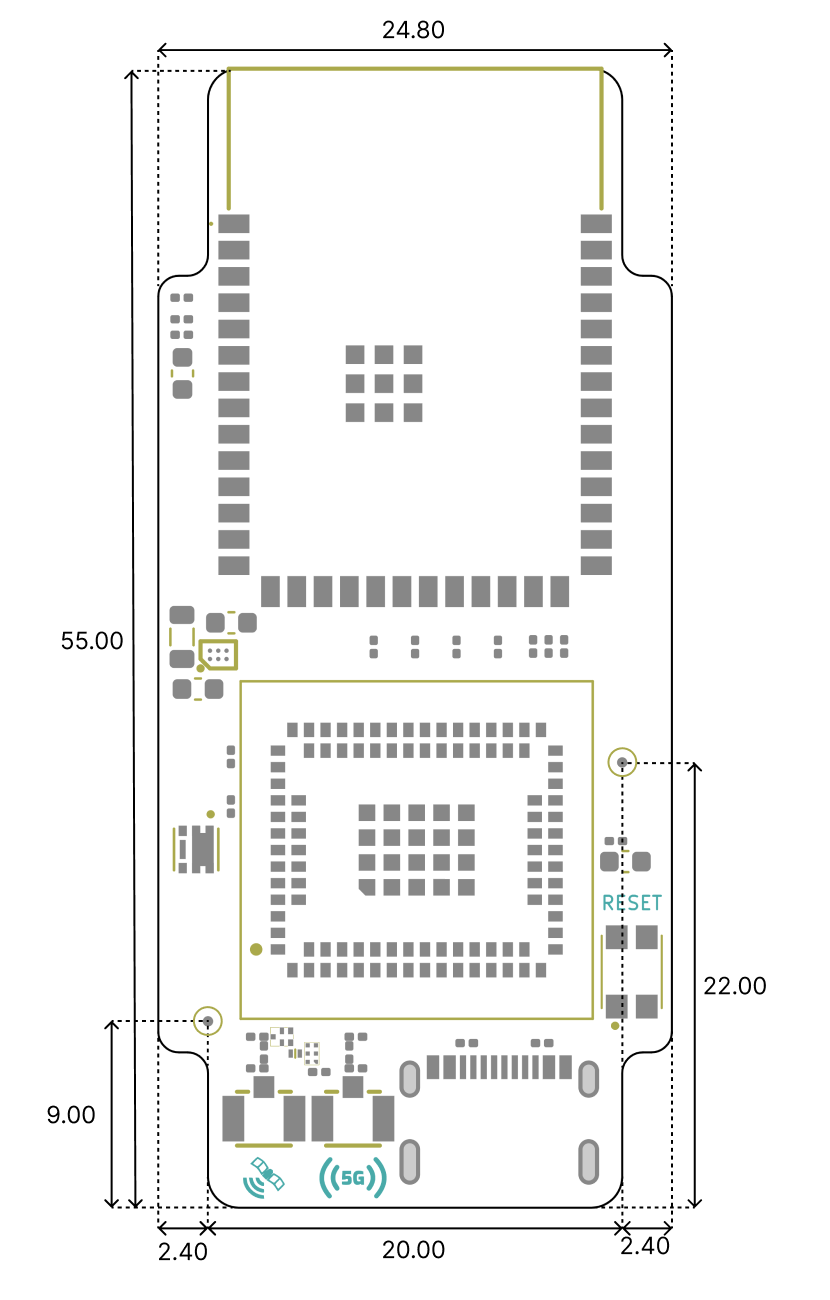
\includegraphics[height=13cm]{mechanical-front.png}
    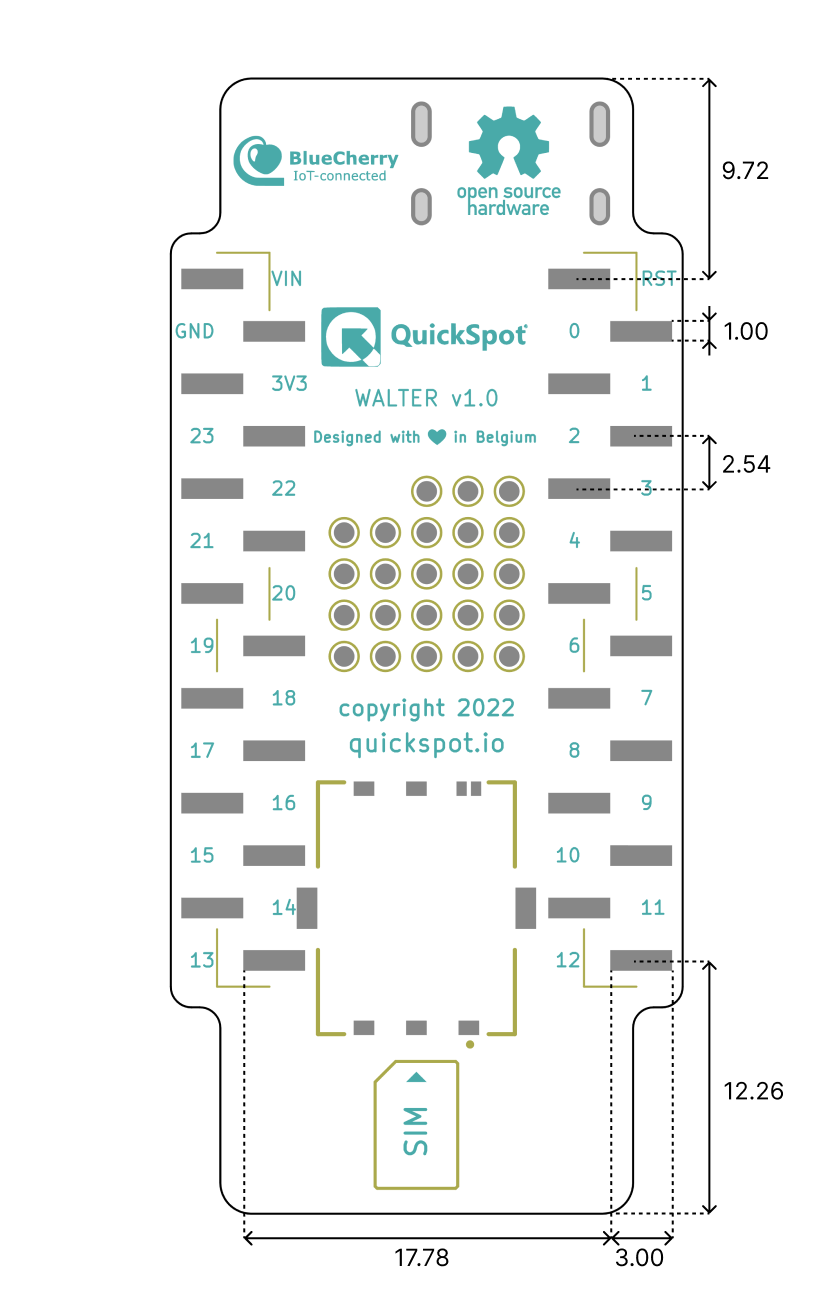
\includegraphics[height=13cm]{mechanical-back.png}
    \caption{Mechanical Drawing Front and Rear View - Unit in mm}
    \label{fig:mechanical_front}
\end{figure}

\section{Software}
\subsection{Libraries and frameworks from QuickSpot}
Walter comes without firmware out of the box. You can easily program and upload your own firmware for Walter using MicroPython, Arduino, ESP-IDF... 
Please refer to the "Getting Started with Walter" available on our GitHub to get you up and running fast.

\subsection{AT commands}

The full set of supported AT commands can be found in the documentation of the Sequans GM02SP. This can be downloaded from this link: \href{https://www.renesas.com/eu/en/document/mah/ryz024-modules-command-users-manual?language=en}{https://www.renesas.com/eu/en/document/mah/ryz024-modules-command-users-manual?language=en}.

\subsection{Manual SFU of the GM02SP}

The second hardware UART of the GM02SP, namely \verb+UART1+, is used for manual firmware upgrades. To do a manual serial SFU of the GM02SP in Walter you must connect \verb+UART1+ via the testpads on the bottom of the module. Use an FTDI UART and make the following connections:
\begin{itemize}
	\item \verb+Walter RX1 <-> FTDI RX+
	\item \verb+Walter TX1 <-> FTDI TX+
	\item \verb+Walter RTS1 <-> FTDI RTS+
	\item \verb+Walter CTS1 <-> FTDI CTS+
	\item \verb+Walter GND <-> FTDI GND+
	\item \verb$Walter Vin <-> +5VDC$
\end{itemize}
Make sure that the 5V power source which is powering Walter and the FTDI share a common ground. To enable smooth updating it is best not to connect the USB-C on Walter to the computer on which the SFU software is running. Now follow the instructions which are bundled with the SFU release.

\section{Operating conditions}
The module can operate in a wide range of temperatures and conditions. The following are guidelines in which the module is guaranteed to work correctly. 
\begin{center}
\renewcommand{\arraystretch}{1.5}
\begin{tabular}{|p{5cm}|c|c|c|c|}
\hline
{\bf Parameter} & {\bf Units} & {\bf Minimum rating} & {\bf Typical rating} & {\bf Maxium rating} \\
\hline
\hline
Working temperature & \textdegree C & -40 &  & 85 \\
\hline
Storage temperature & \textdegree C & -40 &  & 100 \\
\hline
Humidity & \%RH & 10 &  & 90 \\
\hline
Storage humidity & \%RH & 5 & & 90 \\
\hline
\end{tabular}
\end{center}
Please note that no condensation may occur on the PCB and components. 


\section{Legal information}
This module is distributed worldwide by DPTechnics bv. We are not responsible for any product this module is part of. This datasheet is made with great care for detail but it can be possible the datasheet will be updated with more accurate data in te future. Users of DPTechnics bv products can contact us by letter, telephone or email. \\

\noindent DPTechnics bv\\
Westkapellestraat 396/44\\
8300 Knokke-Heist\\
Belgium\\

\noindent Tel: +32(0)50 62 13 79\\
email: info@quickspot.io\\
web: https://www.quickspot.io
\end{document}
